\chapter{File Systems}

\section{Files and file systems}

\begin{definition}
A \textbf{file} is a persistent, named sequence of bytes with associated \textbf{metadata}
(size, owner, permissions, timestamps). A \textbf{file system} is the data structure on a storage
device (and the kernel code) that implements files and directories on top of fixed-size blocks.
\end{definition}

The OS provides a logical view (files, directories, byte offsets) and maps it to the physical
view (block numbers on a device).

\section{File interface}

\begin{lstlisting}[style=c]
int fd = open("/home/vg/notes.txt", O_RDWR | O_CREAT, 0644);
                                       /* returns a file descriptor */
char buf[512];
ssize_t n = read(fd, buf, sizeof buf); /* reads from the current offset */
lseek(fd, 0, SEEK_SET);                /* reposition the offset */
write(fd, "hello", 5);                 /* writes at the current offset */
fsync(fd);                             /* force data to stable storage */
close(fd);
\end{lstlisting}

\begin{itemize}
  \item A \textbf{file descriptor} is a small integer indexing the process's file descriptor
    table. Each entry points to an \emph{open file} object in the kernel holding the current
    \textbf{offset} and access mode, which points to the file's in-memory i-node (vnode).
  \item After \code{fork}, parent and child share open file objects (and therefore offsets).
  \item Reads/writes are \emph{sequential} by default (offset advances); \code{lseek} enables
    random access. Some APIs (\code{pread}/\code{pwrite}) take an explicit offset.
  \item \code{write} usually only updates the in-memory buffer cache; data reaches the disk later
    unless \code{fsync} is called.
\end{itemize}

\begin{figure}[H]
\centering
\begin{tikzpicture}[font=\scriptsize, >=Stealth, x=1cm, y=0.5cm,
  ent/.style={draw, minimum width=0.9cm, minimum height=0.5cm, inner sep=1pt},
  obj/.style={draw, rounded corners, align=center, minimum width=2.2cm, minimum height=0.9cm, inner sep=2pt}]
  \node[font=\small, anchor=east] at (-0.2,2.5) {parent};
  \node[font=\small, anchor=east] at (-0.2,-2.1) {child};
  \foreach \i in {0,...,3} \node[ent] (p\i) at (0.45,4-\i) {\i};
  \foreach \i in {0,...,3} \node[ent] (c\i) at (0.45,-0.6-\i) {\i};
  \node[font=\small] at (4.2,5.0) {open file objects};
  \node[obj, fill=blue!8] (o2) at (4.2,2.6) {offset 0\\mode \code{O\_RDONLY}};
  \node[obj, fill=blue!8] (o1) at (4.2,-1.2) {offset 512\\mode \code{O\_RDWR}};
  \node[font=\small] at (7.9,5.0) {i-nodes (vnodes)};
  \node[obj, fill=green!12] (v2) at (7.9,2.6) {i-node 17};
  \node[obj, fill=green!12] (v1) at (7.9,-1.2) {i-node 42};
  \draw[->] (p2.east) -- (o2.west);
  \draw[->] (c2.east) -- (o2.west);
  \draw[->] (p3.east) -- (o1.west);
  \draw[->] (c3.east) -- (o1.west);
  \draw[->] (o1) -- (v1); \draw[->] (o2) -- (v2);
\end{tikzpicture}
\caption{File descriptors index a per-process table whose entries point to
kernel open-file objects (holding the offset), which point to i-nodes.
After \code{fork}, parent and child share the open-file objects, so a
\code{read} in one advances the offset seen by the other.}
\end{figure}

\section{Directories and links}

Files are organized in a hierarchical namespace: a tree of \textbf{directories}. A directory is
a special file containing \textbf{entries} mapping names to i-node numbers. A \textbf{path}
(\code{/home/vg/notes.txt}) is resolved component by component from the root (absolute) or the
current working directory (relative). \code{.} is the directory itself, \code{..} its parent.

\begin{definition}[Hard link]
A \textbf{hard link} is a directory entry associating a name with an i-node. A file may have
several hard links (in different directories or with different names); all are equally ``the
file''. \code{link(old, new)} adds one, \code{unlink(name)} removes one. The i-node keeps a
\textbf{link count}; the file's data is freed only when the count reaches 0 (and no process has it
open).
\end{definition}
Restrictions: hard links cannot cross file systems (i-node numbers are per file system), and
users may not hard-link directories (to keep the directory structure a tree / DAG without
cycles).

\begin{definition}[Symbolic (soft) link]
A \textbf{symbolic link} is a special file whose content is a path name. When path resolution
reaches it, the kernel substitutes the stored path. Created with \code{symlink(target, name)}.
\end{definition}
Symbolic links can cross file systems and point to directories, but they can \emph{dangle}: if the
target is removed, the link points to nothing. The target's link count does not change.

\begin{example}
\begin{lstlisting}[style=bash]
echo hi > a       # i-node 42, link count 1
ln a b            # hard link: b -> i-node 42, link count 2
ln -s a c         # c is a new i-node whose content is "a"
rm a              # link count 1; b still reads "hi"; c now dangles
\end{lstlisting}
\end{example}

\begin{center}
\begin{tikzpicture}[font=\small, >=Stealth, x=1cm, y=0.8cm,
  de/.style={draw, minimum width=1.2cm, minimum height=0.55cm, font=\ttfamily\small},
  ino/.style={draw, rounded corners, align=center, minimum height=1cm, fill=green!12, font=\scriptsize}]
  \node[font=\scriptsize] at (0,2.1) {directory};
  \node[de, gray, densely dashed] (a) at (0,1.2) {a};
  \node[de] (b) at (0,0.4) {b};
  \node[de] (c) at (0,-0.4) {c};
  \node[ino] (i42) at (3.6,0.8) {i-node 42\\links: 1\\data: \code{hi}};
  \node[ino, fill=orange!15] (i50) at (3.6,-1.0) {symlink i-node\\data: path ``a''};
  \draw[->, gray, densely dashed] (a.east) -- (i42.west) node[pos=0.4, above, font=\tiny]{removed};
  \draw[->, thick] (b.east) -- (i42.west);
  \draw[->, thick] (c.east) -- (i50.west);
  \draw[->, red!70!black, densely dashed] (i50.west) to[out=170, in=0] node[pos=0.6, below, font=\tiny]{} ($(a.east)+(0.05,-0.1)$);
  \node[red!70!black, font=\scriptsize, anchor=west] at (5.0,-1.0) {``a'' no longer exists: dangling};
\end{tikzpicture}
\end{center}
After \code{rm a}: the hard link \code{b} still reaches i-node 42, but the
symbolic link \code{c} stores only the name \code{a}, which no longer
resolves.

\subsection*{Multiple file systems}
Each device/partition holds its own file system. Windows uses drive letters; Unix
\textbf{mounts} a file system at a directory of the existing namespace (\code{mount /dev/sdb1
/mnt/usb}), creating one global tree. OS/161's VFS uses device names (\code{lhd0:}).

\section{File system implementation}

What must be stored on disk:
\begin{itemize}
  \item file data;
  \item file metadata (i-nodes);
  \item directories (names $\to$ i-node numbers);
  \item free-space information for data blocks and i-nodes;
  \item file-system-wide information (the \textbf{superblock}: size, number of i-nodes, location
    of the tables, magic number).
\end{itemize}

\subsection{Very Simple File System (VSFS) layout}
Example from OSTEP: a 256\,KB disk with 4\,KB blocks = 64 blocks.
\begin{center}
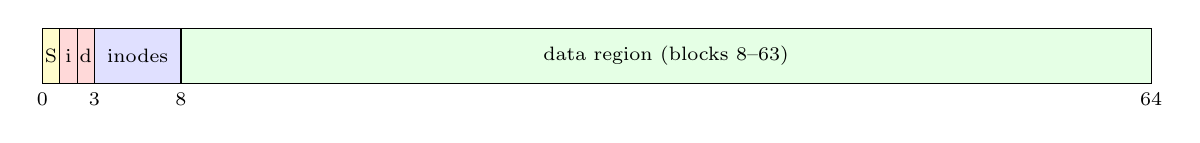
\begin{tikzpicture}[x=0.22cm,y=0.7cm]
  \draw[fill=yellow!20] (0,0) rectangle node{\scriptsize S} (1,1);
  \draw[fill=red!15] (1,0) rectangle node{\scriptsize i} (2,1);
  \draw[fill=red!15] (2,0) rectangle node{\scriptsize d} (3,1);
  \draw[fill=blue!12] (3,0) rectangle node{\scriptsize inodes} (8,1);
  \draw[fill=green!10] (8,0) rectangle node{\scriptsize data region (blocks 8--63)} (64,1);
  \foreach \t in {0,3,8,64} \node[below,font=\scriptsize] at (\t,0) {\t};
\end{tikzpicture}
\end{center}
\begin{itemize}
  \item Block 0: superblock.
  \item Block 1: i-node bitmap (1 bit per i-node: free/used).
  \item Block 2: data bitmap (1 bit per data block).
  \item Blocks 3--7: i-node table. With 256-byte i-nodes, $5 \times 4096/256 = 80$ i-nodes.
  \item Blocks 8--63: data blocks.
\end{itemize}
To find i-node number $k$: block $= 3 + \floor{k \cdot 256 / 4096}$, offset $= (k \cdot 256) \bmod 4096$.

\subsection{I-nodes}
An \textbf{i-node} (index node) is a fixed-size structure holding all metadata of a file
\emph{except its name}: type (file, directory, symlink), permissions, owner, size, link count,
timestamps, and the locations of its data blocks.

\begin{definition}[Indirect blocks]
To support small and large files with a fixed-size i-node, the i-node contains
\begin{itemize}
  \item $D$ \textbf{direct pointers} to data blocks;
  \item a \textbf{single indirect} pointer to a block full of pointers to data blocks;
  \item a \textbf{double indirect} pointer to a block of pointers to single-indirect blocks;
  \item a \textbf{triple indirect} pointer, and so on.
\end{itemize}
\end{definition}

\begin{figure}[H]
\centering
\begin{tikzpicture}[font=\scriptsize, >=Stealth, x=1cm, y=0.45cm,
  ptr/.style={draw, minimum width=1.6cm, minimum height=0.45cm, inner sep=1pt},
  ib/.style={draw, fill=orange!15, minimum width=0.9cm, minimum height=1.05cm, align=center, inner sep=1pt},
  db/.style={draw, fill=green!12, minimum width=0.5cm, minimum height=0.4cm, inner sep=0pt}]
  \node[font=\small] at (0,7.9) {i-node};
  \node[ptr, fill=gray!15, minimum height=0.9cm] at (0,6.2) {metadata};
  \foreach \i/\lab in {0/{direct 0}, 1/{direct 1}, 2/{\ldots}, 3/{direct 11}, 4/{single ind.}, 5/{double ind.}, 6/{triple ind.}}
    \node[ptr] (p\i) at (0,5-\i) {\lab};
  % direct data blocks
  \node[db] (d0) at (2.6,5.6) {}; \node[db] (d1) at (3.2,5.6) {}; \node[db] (d3) at (4.2,5.6) {};
  \node at (3.7,5.6) {\ldots};
  \draw[->] (p0.east) to[out=0, in=-120] (d0.south);
  \draw[->] (p1.east) to[out=0, in=-110] (d1.south);
  \draw[->] (p3.east) to[out=0, in=-100] (d3.south);
  % single
  \node[ib] (s1) at (2.6,1.2) {1024\\ptrs};
  \draw[->] (p4.east) -- (s1.west |- p4);
  \node[db] (sd) at (3.7,1.6) {}; \node[db] (sd2) at (3.7,0.8) {};
  \draw[->] (s1.east |- sd) -- (sd); \draw[->] (s1.east |- sd2) -- (sd2);
  % double
  \node[ib] (d1a) at (2.6,-1.4) {1024\\ptrs};
  \draw[->] (p5.east) -- (d1a.west |- p5);
  \node[ib] (d2a) at (4.2,-1.4) {1024\\ptrs};
  \draw[->] (d1a.east) -- (d2a.west);
  \node[db] (dd) at (5.3,-1.0) {}; \node[db] (dd2) at (5.3,-1.8) {};
  \draw[->] (d2a.east |- dd) -- (dd); \draw[->] (d2a.east |- dd2) -- (dd2);
  % triple
  \node[anchor=west] at (1.9,-3.4) {$\to$ three levels of pointer blocks $\to$ data};
  \draw[->] (p6.east) -- (1.9,-3.4);
\end{tikzpicture}
\caption{An i-node with 12 direct pointers and single, double and triple
indirect pointers (4\,KB blocks, 1024 pointers per block); data blocks are
green, pointer blocks orange. Small files need
only the direct pointers; each extra level multiplies the reach by 1024.}
\end{figure}

\begin{example}[Maximum file size]
4\,KB blocks, 4-byte block pointers ($\Rightarrow$ $P = 1024$ pointers per block), 12 direct
pointers, one single, one double, one triple indirect:
\[
  \text{max blocks} = 12 + 1024 + 1024^2 + 1024^3 \approx 2^{30}, \qquad
  \text{max size} \approx 2^{30} \times 4\,\text{KB} = 4\,\text{TB}.
\]
Reading byte offset $10\,000\,000$: block index $\floor{10^{7}/4096} = 2441$. Since
$2441 \ge 12 + 1024 = 1036$, it is in the double-indirect range at index $2441 - 1036 = 1405$:
first-level slot $\floor{1405/1024} = 1$, second-level slot $1405 \bmod 1024 = 381$. Locating it
needs 3 block reads (double-indirect block, single-indirect block, data) after the i-node.
\end{example}

Alternatives: \textbf{extents} (start block, length) pairs, used by ext4/NTFS, describe large
contiguous files compactly; FAT uses a linked list of blocks stored in a table.

\subsection{Directories on disk}
A directory's data blocks hold entries (i-node number, record length, name length, name).
Looking up a name scans the entries (or uses a hash/B-tree index in modern file systems).
Deleting an entry can leave a gap that is merged into the previous entry's record length.

\subsection{Example: reading \code{/foo/bar}}
\begin{enumerate}
  \item Read the root i-node (number well-known, e.g.\ 2), then root's data block(s) to find
    \code{foo}'s i-node number.
  \item Read \code{foo}'s i-node, then its data to find \code{bar}'s i-node number.
  \item Read \code{bar}'s i-node (permission check, \code{open} returns fd).
  \item Each \code{read()} of a block: read the i-node (block locations), read the data block,
    \emph{write} the i-node (update access time).
\end{enumerate}
Creating a file is worse: read/write the i-node bitmap, write the new i-node, write the
directory data and the directory's i-node, plus data bitmap and data block writes when data is
written. The \textbf{buffer cache} (caching recent blocks in memory) and write-back/delayed
writes absorb most of this traffic.

\subsection{Block allocation}
Free blocks/i-nodes are tracked with bitmaps (or free lists). Allocation policy matters for
performance on HDDs: keep a file's blocks contiguous, and keep files of the same directory close
to each other and to their i-nodes (e.g.\ the Fast File System divides the disk into
\emph{cylinder groups}, each with its own bitmaps, i-nodes and data). Some file systems
pre-allocate several blocks at a time to reduce fragmentation.

\section{Crash consistency}

Updating a file requires several separate disk writes. Example: appending one block to a file
requires writing (1) the data bitmap, (2) the i-node (new pointer, new size), and (3) the data
block. A crash (power loss) can occur between any two writes.

\begin{center}
\begin{tabular}{@{}ll@{}}
\toprule
Writes completed & Result \\
\midrule
data only & no harm (data lost, but FS consistent) \\
i-node only & i-node points to garbage; bitmap says block free (\emph{inconsistent}) \\
bitmap only & space leak: block marked used but no file owns it \\
i-node + bitmap & FS consistent, but file contains garbage \\
i-node + data & inconsistent bitmap (block could be reallocated) \\
bitmap + data & space leak \\
\bottomrule
\end{tabular}
\end{center}

\subsection{fsck}
After an unclean shutdown, a file system checker scans everything: superblock sanity, rebuild
the bitmaps from i-nodes, check link counts against directory entries, find duplicate or bad
block pointers, put orphaned i-nodes in \code{lost+found}. Correct but very slow (time
proportional to disk size, not to the amount of recent work), and it cannot fix ``consistent but
garbage'' cases.

\subsection{Journaling (write-ahead logging)}
Before updating structures in place, first write a description of the update to a
\textbf{journal} (log) area.

\begin{enumerate}
  \item \textbf{Journal write}: write a transaction-begin block (TxB, with a transaction ID),
    then the blocks to be written (e.g.\ new bitmap, i-node, data) to the log.
  \item \textbf{Journal commit}: once those are on disk, write a transaction-end block (TxE,
    a single sector so it is written atomically). The transaction is now durable.
  \item \textbf{Checkpoint}: write the blocks to their real locations.
  \item \textbf{Free}: mark the transaction as done in the journal superblock, so the space can
    be reused.
\end{enumerate}

\begin{figure}[H]
\centering
\begin{tikzpicture}[font=\scriptsize, x=1cm, y=0.8cm, >=Stealth,
  jb/.style={draw, minimum width=1.0cm, minimum height=0.6cm, inner sep=1pt}]
  \node[font=\small, anchor=east] at (-0.2,1) {journal};
  \node[font=\small, anchor=east] at (-0.2,-0.6) {final locations};
  \node[jb, fill=gray!20] at (0.5,1) {TxB};
  \node[jb, fill=blue!10] at (1.5,1) {bitmap};
  \node[jb, fill=blue!10] at (2.5,1) {i-node};
  \node[jb, fill=blue!10] at (3.5,1) {data};
  \node[jb, fill=red!20] at (5.0,1) {TxE};
  \node[jb, fill=blue!10] at (6.8,-0.6) {bitmap};
  \node[jb, fill=blue!10] at (7.8,-0.6) {i-node};
  \node[jb, fill=blue!10] at (8.8,-0.6) {data};
  \draw[decorate, decoration={brace, amplitude=4pt}] (0,1.5) -- (4,1.5) node[midway, above=4pt]{1. journal write};
  \node[above=6pt] at (5.0,1.3) {2. commit};
  \draw[decorate, decoration={brace, amplitude=4pt, mirror}] (6.3,-1.1) -- (9.3,-1.1) node[midway, below=4pt]{3. checkpoint};
  \draw[->, thick, gray] (4.0,0.6) to[out=-30, in=170] (6.3,-0.6);
  \draw[->] (-0.2,-1.8) -- (9.6,-1.8) node[right]{time};
  \draw[densely dashed, red!70!black] (5.6,1.6) -- (5.6,-1.8);
  \node[red!70!black, align=center, anchor=north west] at (5.65,1.6) {crash after here:\\replay};
  \node[gray!50!black, align=center] at (2.2,-0.6) {crash before TxE:\\discard};
\end{tikzpicture}
\caption{Data journaling for one appended block. A crash before the
commit block TxE leaves an incomplete transaction that recovery ignores; a
crash after it is fixed by replaying the logged blocks.}
\end{figure}

Recovery: scan the log; \textbf{replay} (redo) every committed transaction (TxB...TxE complete);
discard incomplete ones. Replaying twice is harmless (redo logging is idempotent). Recovery time
is proportional to the log size, not the disk size.

\begin{important}[Metadata (ordered) journaling]
Data journaling writes every data block twice. Most systems (ext3/ext4 default
``ordered'' mode, NTFS) journal \emph{only metadata}: write the data block to its final location
\emph{first}, then journal and commit the metadata, then checkpoint. This rule ``write the
pointed-to object before the pointer'' guarantees an i-node never points to garbage.
Checksums over the transaction let TxE be written together with the other blocks.
\end{important}

Other approaches: \textbf{soft updates} (carefully order all writes so the on-disk state is
always consistent), \textbf{copy-on-write} file systems (ZFS, btrfs: never overwrite; write new
versions and atomically switch the root pointer), and \textbf{log-structured} file systems
(the whole disk is a log).

\section{OS/161 VFS and SFS}
OS/161 has a virtual file system layer (\code{vfs\_open}, \code{VOP\_READ}, \code{VOP\_WRITE} on
\code{struct vnode}) that hides differences between file systems: \code{emufs} (passes calls to
the host file system) and \code{SFS}, a simple Unix-like file system with a superblock, a
free-block bitmap, i-nodes with direct and single-indirect pointers, and directories of
fixed-size entries. Data moves between kernel and user space with \code{struct uio}.

\section*{Summary}
\begin{itemize}
  \item Files: named, persistent byte sequences with metadata; accessed through file
    descriptors and per-open offsets.
  \item Directories map names to i-node numbers. Hard links share an i-node (link count);
    symbolic links store a path and can dangle.
  \item On disk: superblock, i-node and data bitmaps, i-node table, data blocks (VSFS).
  \item I-nodes locate data with direct, single, double, triple indirect pointers.
  \item Multi-write updates are vulnerable to crashes; fsck repairs slowly, journaling commits
    updates atomically to a log and replays committed transactions after a crash.
\end{itemize}
